\documentclass[12pt,a4paper,bibliography=totocnumbered,listof=totocnumbered]{scrartcl}
\usepackage[ngerman]{babel}
\usepackage[utf8]{inputenc}
\usepackage{amsmath}
\usepackage{amsfonts}
\usepackage{amssymb}
\usepackage{graphicx}
\usepackage{fancyhdr}
\usepackage{tabularx}
\usepackage{geometry}
\usepackage{setspace}
\usepackage[right]{eurosym}
\usepackage[printonlyused]{acronym}
\usepackage{subfig}
\usepackage{floatflt}
\usepackage[usenames,dvipsnames]{color}
\usepackage{colortbl}
\usepackage{paralist}
\usepackage{array}
\usepackage{titlesec}
\usepackage{parskip}
\usepackage[right]{eurosym}

\usepackage[subfigure,titles]{tocloft}
\usepackage[pdfpagelabels=true]{hyperref}

\usepackage{listings}
\lstset{basicstyle=\footnotesize, captionpos=b, breaklines=true, showstringspaces=false, tabsize=2, frame=lines, numbers=left, numberstyle=\tiny, xleftmargin=2em, framexleftmargin=2em}
\makeatletter
\def\l@lstlisting#1#2{\@dottedtocline{1}{0em}{1em}{\hspace{1,5em} Lst. #1}{#2}}
\makeatother

\geometry{a4paper, top=27mm, left=30mm, right=20mm, bottom=35mm, headsep=10mm, footskip=12mm}

\hypersetup{unicode=false, pdftoolbar=true, pdfmenubar=true, pdffitwindow=false, pdfstartview={FitH},
	pdftitle={Projektkurs Dokumentation},
	pdfauthor={Jakob Fleischer, Robin Schlaak, Lars Schmalbach},
	pdfsubject={Dokumentation},
	pdfcreator={\LaTeX\ with package \flqq hyperref\frqq},
	pdfproducer={pdfTeX \the\pdftexversion.\pdftexrevision},
	pdfkeywords={Dokumentation},
	pdfnewwindow=true,
	colorlinks=true,linkcolor=black,citecolor=black,filecolor=magenta,urlcolor=black}
\pdfinfo{/CreationDate \today}

\begin{document}

\titlespacing{\section}{0pt}{12pt plus 4pt minus 2pt}{-6pt plus 2pt minus 2pt}

% Kopf- und Fusszeile
\renewcommand{\sectionmark}[1]{\markright{#1}}
\renewcommand{\leftmark}{\rightmark}
\pagestyle{fancy}
\lhead{}
\chead{}
\rhead{\thesection\space\contentsname}
\lfoot{Dokumentation unseres Projekts\newline im Projektkurs Mathe-Physik-Informatik}
\cfoot{}
\rfoot{\ \linebreak Seite \thepage}
\renewcommand{\headrulewidth}{0.4pt}
\renewcommand{\footrulewidth}{0.4pt}

% Vorspann
\renewcommand{\thesection}{\Roman{section}}
\renewcommand{\theHsection}{\Roman{section}}
\pagenumbering{Roman}

% ----------------------------------------------------------------------------------------------------------
% Titelseite
% ----------------------------------------------------------------------------------------------------------
\thispagestyle{empty}
\begin{center}
	
\includegraphics[scale=2]{Bilder/aeg-logo.png}\\
	
	\Large
	\textbf{Albert-Einstein-Gymnasium}\\
	\vspace*{2cm}
	\vspace*{2cm}
	\Huge
	\textbf{Dokumentation}\\
	\vspace*{0.5cm}
	\large
	zu unserem Projekt im Projektkurs\\
	\vspace*{1cm}
	\Huge
	\textbf{Mathe-Physik-Informatik}\\
	\vspace*{2cm}
	
	\vfill
	\normalsize
	\newcolumntype{x}[1]{>{\raggedleft\arraybackslash\hspace{0pt}}p{#1}}
	\begin{tabular}{x{6cm}p{7.5cm}}
		\rule{0mm}{5ex}\textbf{Autoren:} & Jakob Fleischer\newline Robin Schlaak \newline
		Lars Schmalbach \\ 
		\rule{0mm}{5ex}\textbf{Prüfer:} & Herr Thomas Bachran \\ 
		\rule{0mm}{5ex}\textbf{Abgabedatum:} & 21.06.2017 \\ 
	\end{tabular} 
\end{center}
\pagebreak

% ----------------------------------------------------------------------------------------------------------
% Abstract
% ----------------------------------------------------------------------------------------------------------
\setcounter{page}{1}
\onehalfspacing
\titlespacing{\section}{0pt}{12pt plus 4pt minus 2pt}{2pt plus 2pt minus 2pt}
\rhead{KURZFASSUNG}
\section{Umschreibung des Projekts}
\emph{Jakob}
\\
Die grundsätzliche Zielsetzung von unserem Projekt war, etwas zu programmieren, das
wir auch selber danach noch sinnvoll nutzen können.
Ein Projekt zu finden, dass dieses Ziel erfüllte und für uns innerhalb eines Schuljahres realisierbar gewesen wäre, gestaltete sich jedoch als schwierig, da wir zwar alle drei bereits Programmiererfahrung besaßen, diese sich jedoch auf das Programmieren einfacher Klassenstrukturen mit Rückgabewerten in der Eclipse-Konsole
beschränkte.
Also mussten wir, begründet auf diesen Fakt, unsere Fähigkeit ein selbständiges Programm zu schreiben, zu diesem Zeitpunkt, realistisch, als nicht vorhanden einschätzen.

Dieses Eingeständnis blies uns recht schnell die Traumwolke eines Programms, welches mithilfe einer künstlichen Intelligenz Bilder auswertet, unter den Füßen weg und ließ uns den festen Boden der Tatsachen unter denselbigen spüren.
Aus diesem Grund kamen wir zu dem Schluss, dass eine Software, die Dateien sämtlicher Dateitypen automatisch und sortiert abspeichert, als ein sinnvolles und zugleich erreichbares erstes Ziel, welches wir dann gut ausbauen könnten.
Jedoch haben wir uns auch in diesem Punkt selber überschätzt.

Wir haben zwar unser Ziel eines webbasierten Programms zur sortierten Abspeicherung von Dateien erreicht, jedoch hat alleine dieses \glqq erste Ziel\grqq{} unsere gesamte zeitliche Kapazität verschlungen, ohne uns Zeit für Erweiterungen zu lassen.
Doch dazu mehr in der folgenden detaillierten Dokumentation unseres Kampfes mit Computern, Quellcodes und vor allem mit uns selbst.

\vspace{-1,2em}
\titlespacing{\section}{0pt}{12pt plus 4pt minus 2pt}{-6pt plus 2pt minus 2pt}

\pagebreak

% ----------------------------------------------------------------------------------------------------------
% Verzeichnisse
% ----------------------------------------------------------------------------------------------------------
% TODO Typ vor Nummer
\renewcommand{\cfttabpresnum}{Tab. }
\renewcommand{\cftfigpresnum}{Abb. }
\settowidth{\cfttabnumwidth}{Abb. 10\quad}
\settowidth{\cftfignumwidth}{Abb. 10\quad}

\titlespacing{\section}{0pt}{12pt plus 4pt minus 2pt}{2pt plus 2pt minus 2pt}
\singlespacing
\rhead{INHALTSVERZEICHNIS}
\renewcommand{\contentsname}{II Inhaltsverzeichnis}
\phantomsection
\addcontentsline{toc}{section}{\texorpdfstring{II \hspace{0.35em}Inhaltsverzeichnis}{Inhaltsverzeichnis}}
\addtocounter{section}{1}
\tableofcontents
\pagebreak


\rhead{VERZEICHNISSE}
\listoffigures
\pagebreak
\listoftables
\pagebreak
\renewcommand{\lstlistlistingname}{Listing-Verzeichnis}
{\labelsep2cm\lstlistoflistings}
\pagebreak

% ----------------------------------------------------------------------------------------------------------
% Abkürzungen
% ----------------------------------------------------------------------------------------------------------
%\section{Abkürzungsverzeichnis}
%\begin{acronym}[OSGi] % längste Abkürzung steht in eckigen Klammern
%	\setlength{\itemsep}{-\parsep} % geringerer Zeilenabstand
%	\acro{OSGi}{Open Service Gateway initiative}
%\end{acronym}
%\newpage

% ----------------------------------------------------------------------------------------------------------
% Inhalt
% ----------------------------------------------------------------------------------------------------------
% Abstände Überschrift
\titlespacing{\section}{0pt}{12pt plus 4pt minus 2pt}{-6pt plus 2pt minus 2pt}
\titlespacing{\subsection}{0pt}{12pt plus 4pt minus 2pt}{-6pt plus 2pt minus 2pt}
\titlespacing{\subsubsection}{0pt}{12pt plus 4pt minus 2pt}{-6pt plus 2pt minus 2pt}

% Kopfzeile
\renewcommand{\sectionmark}[1]{\markright{#1}}
\renewcommand{\subsectionmark}[1]{}
\renewcommand{\subsubsectionmark}[1]{}
\lhead{Kapitel \thesection}
\rhead{\rightmark}

\onehalfspacing
\renewcommand{\thesection}{\arabic{section}}
\renewcommand{\theHsection}{\arabic{section}}
\setcounter{section}{0}
\pagenumbering{arabic}
\setcounter{page}{1}

% ----------------------------------------------------------------------------------------------------------
% Einleitung
% ----------------------------------------------------------------------------------------------------------
\section{Kapitel: Herangehensweise}
\emph{Jakob}\\
Dieses Kapitel soll sich primär mit uns beschäftigen.
Damit, wie wir an die Projektarbeit herangetreten und auch wo wir auf Probleme mit derselben gestoßen sind.

\subsection{ursprüngliche Vorstellung und Konsequenzen}
\emph{Jakob}\\
Unsere Unerfahrenheit in der Projektarbeit hat uns zu einem überstürzten und unüberlegten Projekteinstieg getrieben, bei dem wir uns in Themen eingearbeitet haben, ohne uns einen genauen Plan zu erstellen.
Dies führte zu einer eher mäßig koordinierten Arbeitsteilung, deren Teilung in absoluter Trennung bestand, wodurch bereits nach kurzer Zeit keiner mehr wusste, was seine Themen mit denen der Anderen, geschweige denn, mit unserem Projekt zu tun hatten.
Jedoch unterdrückten wir, aus der naiven Vorstellung heraus, dass die Anderen schon wissen, was sie tun, und dass das schon alles noch Sinn ergeben wird, diese Zweifel und arbeiteten weiter, ohne uns über die Folgen dieser schlechten Kommunikation untereinander im Klaren zu sein.

\subsection{verspätete Planung}
\emph{Lars}\\
Zu spät haben wir gemerkt, dass unsere bisherige Arbeit weder zielführend, noch in irgendeiner Weise sinnvoll war, weshalb wir uns zusammengesetzt und intensiv beraten haben. Aus dieser Beratung entstand zum ersten Mal ein und realistischer Plan bezüglich des Aufbaus unseres Programms. Auch die Aufteilung der verschiedenen Arbeitsschritte zwischen den  drei Gruppenmitgliedern fand hier spezifisch statt.

\subsubsection{Aufteilung}
\label{sec:Aufteilung}

\vspace{1em}
\begin{minipage}{\linewidth}
	\centering
	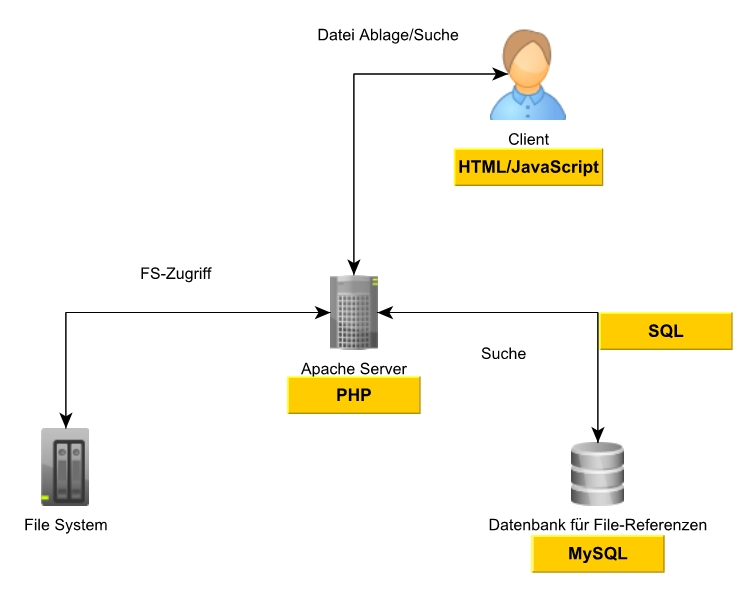
\includegraphics[width=0.7\linewidth]{Bilder/Projekt-Entwurf.jpg}
	\captionof{figure}[Erster realistischer Plan]{Erster realistischer Plan}
	\label{fig:plan1}
\end{minipage}
\vspace{1em}

In Abbildung \ref{fig:plan1} wird die Aufteilung der verschiedenen Aufgaben dargestellt. Der Client [\ref{sec:Client / GUI}], welcher von Lars programmiert werden sollte, umfasst allgemein gesagt dass GUI, also die Benutzeroberfläche, und dessen Kommunikation mit dem Server. Dieser wiederum soll von Robin eingerichtet und so gestaltet werden, dass er Anfragen kategorisiert und je nach Art der Anfrage das Datei-System beziehungsweise die Datenbank anspricht. Die soeben erwähnte Datenbank wird von Jakob erstellt und soll zunächst nur die Referenzen zu den Dateien im Datei-System abspeichern und verwalten.\\

\subsubsection{Client / GUI}
\label{sec:Client / GUI}

Die Tabelle \ref{tab:PlanungClient} ist die digitalisierte Version des Tafelbilds, welches bei der oben beschriebenen, intensiven Beratung entstanden ist. Grün steht dabei dafür, dass diese Kriterien automatisch erkannt werden sollen, rot markierte sollen erfragt werden und das blau markierte Kriterium ist eine optionale Angabe. Hierbei ist zu beachten, dass bei der Suche alle Angaben optional sind, sodass man, wenn man eine Suche ohne Kriterien startet, alle vorhandenen Dateien als Ergebnis ausgegeben bekommt.

\vspace{1em}
\begin{table}[!h]
	\centering
	\begin{tabular}{|p{3.3cm}|p{3.3cm}|p{3.3cm}|p{3.3cm}|}
		\hline
			\begin{center}
				\textbf{Ablage}
			\end{center}
			&
			\begin{center}
				\textbf{Suchen}
			\end{center}
			&
			\begin{center}
				\textbf{Löschen}
			\end{center}
			&
			\begin{center}
				\textbf{Ändern}
			\end{center}
		\\
		\hline
			\begin{itemize}[]
				\item[-]\textcolor{ForestGreen}{Typ}
				\item[-]\textcolor{ForestGreen}{Größe}
				\item[-]\textcolor{red}{Datei}
				\item[-]\textcolor{red}{Name}
				\item[-]\textcolor{red}{Datum}
				\item[-]\textcolor{blue}{zusätzliche Info}
			\end{itemize}
			&
			\begin{itemize}[]
				\item[]Kriterien:
				\item[-]\textcolor{red}{Name}
				\item[-]\textcolor{red}{Inhalt}
				\item[-]\textcolor{red}{Typ}
				\item[-]\textcolor{red}{Datum}
				\item[-]\textcolor{red}{Ort}
			\end{itemize}
			&
			\begin{itemize}[]
				\item[-]verbunden mit Suche
				\item[-]senden eines Löschbefehls
			\end{itemize}
			&
			\begin{itemize}[]
				\item[]Beinhaltet:
				\item[-]Suche
				\item[-]Ändern
				\item[-]Ablage
			\end{itemize}
			\\
		\hline
	\end{tabular}
	\caption{Planung des GUIs und dessen Funktionen}
	\label{tab:PlanungClient}
\end{table}

\subsubsection{Server}
\label{sec:Server}
Auch die Aufgaben des Servers wurden in unserem Tafelbild aufgeführt. Diese werden in Tabelle \ref{tab:PlanungServer} dargestellt.

\vspace{1em}
\begin{table}[!h]
	\centering
	Aufgaben des Servers in Verbindung mit...\\
	\begin{tabular}{|p{4cm}|p{4cm}|p{4cm}|}
		\hline
			\begin{center}
				\textbf{Client}
			\end{center}
			&
			\begin{center}
				\textbf{Datei-System}
			\end{center}
			&
			\begin{center}
				\textbf{Datenbank}
			\end{center}
		\\
		\hline
			\begin{itemize}[]
				\item[-]Auswerten der Metadaten bei der Ablage
				\item[-]Auswerten von Suchkriterien
				\item[-]Senden von Dateien bei der Suche
			\end{itemize}
			&
			\begin{itemize}[]
				\item[-]Ablage
				\item[-]Abruf
				\item[-]Löschen
			\end{itemize}
			&
			\begin{itemize}[]
				\item[-]Erstellen der Datenbank, falls keine vorhanden ist
				\item[-]Referenzen senden und erhalten
				\item[-]Einträge löschen
			\end{itemize}
		\\
		\hline
	\end{tabular}
	\caption{Planung des Servers}
	\label{tab:PlanungServer}
\end{table}

\subsubsection{Datenbank}
\label{sec:Datenbank}
Die Datenbank, so nahmen wir es uns vor, soll Dateien aufnehmen und den Abfragen entsprechend antworten. Beinhalten sollte sie zunächst nur den Dateinamen, sowie weitere Attribute, welche in Tabelle [\ref{tab:PlanungClient}] aufgeführt sind. Zusätzlich soll zu jeder Datei noch der jeweilige  Pfad gespeichert werden, sodass ein Zugriff auf die Datei gewährleistet werden kann.


\subsection{Zusammenarbeit und Kommunikation}
\emph{Jakob}\\
Wie bereits bei unseren Vorstellungen erwähnt [siehe [\ref{sec:Vorstellung}]], ist unsere Projektarbeit haupt- sächlich negativ durch unser Kommunikationsverhalten beeinflusst worden.
Unser größtes Problem lag in der Organisation unserer Zusammenarbeit. Dies ist der Tatsache verschuldet gewesen, dass wir in der Schule meist nur unter strengen Regulierungen und Vorgaben arbeiten, weshalb so ein freies und selbständiges Arbeiten sehr ungewohnt für uns war und vielerorts neben den anderen Arbeiten, bei denen bei \glqq Nicht-Erfüllen\grqq{} direkte Sanktionen drohten, an Priorität zu verlieren schien.
Aus diesem Grund war unsere Zusammenarbeit größtenteils von stark differenzierenden Arbeitshaltungen geprägt, welche sich dann auch auf die Aktivität und Harmonie unserer Kommunikation untereinander ausgeprägt haben.
Dies begünstigte unseren fehlgeleiteten Ansatz [siehe [\ref{sec:Vorstellung}]] und führte auch in der späteren Projektarbeit immer wieder zu Einbrüchen unserer Produktivität, welche im Nachhinein als vermeidbar und gar unnötig einzustufen sind.

\pagebreak
% ----------------------------------------------------------------------------------------------------------
% Grundlagen
% ----------------------------------------------------------------------------------------------------------

\section{Kapitel: Grundlagen}
\emph{Jakob \emph{\&} Lars}\\
Im zweiten Kapitel dieser Dokumentation wird genauer auf die Themen eingegangen, in welche wir uns im Laufe des Projektkurses hineingearbeitet haben. Es wird nicht nur auf für das Projekt relevante Techniken, sondern auch auf solche, in die wir uns zwar eingearbeitet haben, sie jedoch nicht verwendet haben, eingegangen.

\subsection{LaTeX}
\label{sec:LaTeX}
\emph{Robin}\\
LaTeX ist ein softwarepaket, welches die Benutzung des Textsatzsystems TeX vereinfacht. LaTeX wurde Anfang der 1980er von dem Programierer, Mathematiker und Informatiker Leslie Lamport entwickelt.\cite{LaTeX}\cite{Lamport}
...

\subsection{XAMPP}
\label{sec:XAMPP}
\emph{Robin}\\
Xampp ist ein Softwarepaket bestehend aus Freeware. Xampp vereinfacht das Instelliernen und das Konfigurieren von einem Apache Webservers mit z.B. SQLite und PHP. Außerdem sind in Xampp noch Werkzeuge wie z.B. FileZilla und phpMyAdmin vorhanden. Xampp ist nnicht für den Einsatz bei öffenliche Server gedacht, sondern dient lediglich für Entwickler, die ein schnelles und kompaktes Testsystem haben wollen, da eine starke Einschränkung der Sicherheit gibt.\cite{XAMPP}

...

\subsection{HTML}
\label{sec:HTML}
\emph{Lars}\\
HTML ist die Abkürzung für \glqq Hypertext Markup Language\grqq, was zu deutsch \glqq Hypertext-Auszeichnungssprache\grqq{} heißt. Es ist eine Programmiersprache, mit der man den Aufbau von Internetseiten bestimmt. Solche HTML-Dokumente stellen die Grundlage für das World Wide Web dar und werden von Browsern dargestellt.\cite{HTML}\cite{Hypertext_Markup_Language} Sie bestehen in der Regel aus drei Teilen.\cite{HTML/Dokumentstruktur_und_Aufbau} 

\vspace{1em}
\begin{lstlisting}[caption= Beispiel für ein einfaches HTML-Dokument, label=lst:HTML]
<html>
	<head>
		<meta charset="UTF-8">		
		<title> Titel</title>
	</head>
	<body>
		Sichtbarer Text auf der Webseite.
	</body>
</html>
\end{lstlisting}

Der erste Teil eines üblichen HTML-Dokuments ist die Dokumenttyp-Deklaration. In ihr werden Angaben zur verwendeten HTML-Version gegeben. Im \glqq head\grqq , welcher den zweiten Teil darstellt, werden  Kopfdaten, wie zum Beispiel der Titel der Seite oder andere, für den menschlichen Betrachter der Webseite zunächst nicht sichtbare, Informationen zur korrekten Darstellung des sichtbaren Teils der Webseite, angegeben.\cite{HTML/Kopfdaten} Anzuzeigende Inhalte werden in den \glqq body\grqq{}, den dritten Teil, geschrieben. Hier werden also sämtliche Texte, Verweise, Grafiken und so weiter eingefügt, die auf der Webseite sichtbar sein sollen.\cite{HTML/Dokumentstruktur_und_Aufbau} \\
In unserem Fall stellt HTML die Grundlage für die optische Gestaltung des GUIs dar.

\subsubsection{Frames}
\label{sec:Frames}
Eine hilfreiche Technik, die auch bei uns ihren Einsatz gefunden hat, heißt Frames. Diese Technik wurde 1996 von Netscape eingeführt. Mit ihr kann man mehrere Dateien gleichzeitig auf dem Bildschirm anzeigen lassen.\cite{HTML/Frames} Sie wurde jedoch im Oktober 2014 mit HTML5\cite{HTML5} aus dem Standard entfernt, da sie entscheidende Nachteile aufweist. Aufgrund des Verwendungszweckes unserer Webseite benutzen wir Frames, obwohl empfohlen wird, Server-seitig andere Techniken zum Auslagern von Teilen der Seite zu benutzen.\cite{HTML/Frames} Die stärksten Argumente waren, die simple Handhabung und die guten Gestaltungsmöglichkeiten mit dieser Technik. \\
Im Folgenden Beispiel wird ein sogenanntes Frameset dargestellt, bei dem der Bildschirm, mit dem Attribut \glqq rows\grqq{} in zwei Zeilen aufgeteilt wird, wobei die obere 20\% der Pixel einnimmt und die untere den Rest, also 80\%. Alternativ kann man den Bildschirm auch in Spalten aufteilen, dies geschieht mit dem Attribut \glqq cols\grqq . Des Weiteren wird mit dem Attribut \glqq border\grqq{} die Breite des Randes zwischen den jeweiligen Frames angegeben.

\vspace{1em}
\begin{lstlisting}[caption= Beispiel für Frames in HTML, label=lst:HTML]
<html>
	<head>
		<title>Titel</title>
	</head>
	<frameset rows="20%,*" border="1">
		<frame src="Quelle1.html">
		<frame src="Quelle2.html">
	</frameset>
</html>
\end{lstlisting}

\subsubsection{Tabellen}
\label{sec:Tabellen}
Tabellen in HTML [\ref{sec:HTML}] bieten gute, einfache und vielseitige Möglichkeiten, Internetseiten zu strukturieren. Sie wurden im Januar 1997 mit HTML 3.2 ins Standardrepertoire von HTML aufgenommen.\cite{Hypertext_Markup_Language} \\
Das Folgende Beispiel beinhaltet eine Tabelle mit zwei Zeilen und zwei Spalten. Tabellen in HTML werden Zeile für Zeile definiert. Eine Zeile beginnt mit $<$tr$>$ und wird mit $<$/tr$>$ beendet. Mithilfe der Befehle $<$td$>$ und $<$/td$>$ werden die Tabelleneinträge, also die Spalten in den jeweiligen Zeilen, definiert.

\vspace{1em}
\begin{lstlisting}[caption= Beispiel für Tabellen in HTML, label=lst:HTML]
<html>
	<head>
		<meta charset="UTF-8">		
		<title> Titel</title>
	</head>
	<body>
		<table>
			<tr>
				<td>
					Oben links
				</td>
				<td>
					Oben rechts
				</td>
			</tr>
			<tr>
				<td>
					Unten links
				</td>
				<td>
					Unten rechts
				</td>
			</tr>
		</table>
	</body>
</html>
\end{lstlisting}

\subsubsection{Formulare}
\label{sec:Formulare}
Formulare sind ein Element von HTML, [\ref{sec:HTML}] das es ermöglicht Daten zu erfassen und über das Hypertext Transfer Protocol per XMLHttpRequest, HTTP-GET oder HTTP-POST zur Verarbeitung an einen Server zu senden.\cite{Webformular} In unserem Programm kam letzteres zum Einsatz. Man kann in HTML zwar Formulare definieren und erstellen, für eine Verarbeitung und Auswertung der Eingaben ist jedoch eine andere Programmiersprache, wie zum Beispiel Javascript [\ref{sec:JavaScript}] oder PHP [\ref{sec:PHP}] nötig.\cite{HTML/Formulare/Form} \\
In unserem Fall haben wir Formulare in Form von Anmeldeformularen, Suchfiltern und auch als Möglichkeit zum Hochladen von Dateien eingesetzt.\\
In dem folgenden Beispiel ist die Implementation eines Formulars in HTML dargestellt. Zu sehen ist ein Formular, welches ein Label, also den Text \glqq Suchgbegriff\grqq{} enthält. Die Zugehörigkeit des darauf folgenden Eingabefelds zum Label wird durch das Attribut \glqq name\grqq{} festgelegt. Das zweite \glqq input\grqq{} Statement erstellt den Bestätigungsknopf, den man drücken muss, um das Formular abzusenden. Beim Absenden des Formulars wird die Datei oder die Internetseite aufgerufen, die im Kopf des Formulars unter dem Attribut \glqq action\grqq{} steht.

\vspace{1em}
\begin{lstlisting}[caption= Beispiel für Formulare in HTML, label=lst:HTML]
<html>
	<head>
		<title>
			Titel
		</title>
	</head>
	<body>
		<form action="action.php">
 			 <label for="begriff">Suchbegriff</label>
	 		 <input type="text" name="begriff">
	 		 
	 		 <input type="submit" name="Submit" value="Suchen">
		</form>
	</body>
</html>
\end{lstlisting}

\subsubsection{JavaScript}
\label{sec:JavaScript}
Bei JavaScript handelt es sich um eine interpretierende Programmier- beziehungsweise Skriptsprache, die 1995 von Netscape entwickelt wurde.\cite{JavaScript}\cite{wiki/JavaScript} JavaScript ist sehr verbreitet, da sich in allen modernen Browsern Interpreter für die Sprache befinden. Es wird hauptsächlich Client-seitig verwendet und ermöglicht es, dynamischen Einfluss auf Webseiten zu nehmen.\cite{JavaScript-JS} Für unser Programm kam die Sprache besonders häufig aufgrund des, durch sie ermöglichten, einfachen Umgangs mit Variablen und Funktionen zum Einsatz.

\subsection{PHP}
\label{sec:PHP}
\emph{Robin}\\
PHP (Hypertext Preprocessor, ursprünglich: Personal Home Page) ist eine Skriptsprache welche huptsöchlich zur erstellung dynamischer Webseiten und Webanwendungen genutzte wird. Und damit eine Art Erweiterung von HTML. Der Syntax von PHP ist dem von C und Perl angelent. PHP zeichnet sich durch Internet-Protokolleinbindung und Datenbankunterstützung.
 \cite{PHP}


\subsubsection{GET-/POST-Methoden}
\emph{Robin}\\
Die POST-Mehtode wir häufig eingesetzt, um eine Anfrage des Clients mit weiteren Daten, an den Server weiter zu geben. POST hat die Funktionen einen Datenblock mit dazugehörigen Informationen und die Funktion Nnchrichtin zu übertragen. Dies Mit hilfe der URI.

Die GET-MEthode hat die Möglichkeit Informationen jeglicher Art zu identifizieren. Dies auch mit hilfe der Ergebnis-URI.
\cite{GETPOST}

\subsection{Apache HTTP Server}
\label{sec:Apache}
\emph{Lars}\\
Bei dem Apache HTTP Server handelt es sich um den seit 1996 verbreitetsten Webserver der Welt. Er war das Gründungsprojekt der Apache Software Foundation und wurde im April 1995 veröffentlicht. Ursprünglich ist er eine gepatchte Erweiterung des bereits etablierten NCSA HTTP Servers. Im März 2000, also knapp 5 Jahre nach der Veröffentlichung der ersten Version wurde Apache 2.0 veröffentlicht. Es wurden sowohl die Stabilität, als auch die Geschwindigkeit verbessert. Die aktuellste Version, welche auch von den Entwicklern zur Benutzung empfohlen wird, ist die Version 2.4.25, welche am 20.06.2016 veröffentlicht wurde.\cite{wiki/Apache_HTTP_Server}\cite{apache.org}\\
Allgemein haben Webserver, sowie auch der Apache HTTP Server, die Hauptaufgabe, statische Dateien an Clients, wie zum Beispiel Webbrowser, zu übertragen. \cite{Webserver}\\
Auch der Apache HTTP Server, der in unserem Programm zum Einsatz kommt muss solche Dateien, hauptsächlich HTML- und PHP-Dokumente, [\ref{sec:HTML}][\ref{sec:PHP}] verwalten und entsprechend zur Verfügung stellen. Wir benutzen den Apache HTTP Server, in Verbindung mit XAMPP, [\ref{sec:XAMPP}] da dieses die Installation, Konfiguration und Verwaltung des Servers erheblich vereinfacht.

\subsection{Editoren und integrierte Entwicklungsumgebungen}
\label{sec:Editoren}
\emph{Lars}\\
Editoren werden zum Schreiben von Texten, wie zum Quellcodes, benutzt. gute Editoren helfen das Programmieren zu vereinfachen, indem sie gewisse Schlüsselwörter, sowie Befehle, farblich hervorheben, eine Autovervollständigung, eine Such- und Ersetzfunktion und indem sie den Quellcode automatisch einrücken. Zusätzlich stellen sie eine Schnittstelle für Plugins dar.\cite{Texteditor} \\
Neben Editoren gibt es auch integrierte Entwicklungsumgebungen. Diese bestehen aus einer Sammlung an Computerprogrammen, mit denen es möglich ist Software ohne die Verwendung vieler einzelner Programme zu entwickeln. Durch sie werden nicht nur Tippfehler verhindert, sondern auch Arbeitsschritte und somit Zeit bei der Softwareentwicklung gespart.\cite{Integrierte_Entwicklungsumgebung}\cite{Medienbruch}
Bei der Entwicklung unseres Programms kamen die Editoren und integrierten Entwicklungsumgebungen Eclipse [\ref{sec:Eclipse}] (genau genommen Eclipse Neon IDE), Notepad++ [\ref{sec:Notepad++}] und Texmaker [\ref{sec:Texmaker}] zum Einsatz.

\subsubsection{Eclipse}
\label{sec:Eclipse}
\emph{Robin}\\
Eclipse ist eine Freeware und dient als Programierwerkzeug zur Entwicklung diverser Software. Früher wurde Eclipse als integrierte Entwicklungsumgebung (IDE) für Java genutzt. Mittlerweile wird eclipse wegen seiner Erweiterbarkeit auch für viele andere diverse Entwicklungsaufgaben genutzt. Eclipse ist der Nachfolger von IBM Visual Age for Java 4.0. Seit dem 7. Novermber 2001 ist der Quellcode für Eclipse freigegeben. \cite{Eclipse}
...

\subsubsection{Notepad ++}
\label{sec:Notepad++}
\emph{Robin}\\
Notepad ++ ist eine Freeware und ein Texteditor für Windows. In Notepad++ kann man mit vielen verschiedenen Programiersprachen schreiben, es werden auch deren Syntax und Struktur hervorgehoben. Notepad++ selbst ist in C++ geschrieben. \cite{Notepad}
...

\subsubsection{Texmaker}
\label{sec:Texmaker}
\emph{Robin}\\
TeXmaker ist ein Unicode-Texteditor für das Erstellen von LaTeX-Dokumenten. Dieser Editor richtet sich insbesondere an LaTeX-Anfänger, da durch Assistenten die Erstellung von Dokumenten vereinfacht wird. \cite{Texmaker}
...

\subsection{GitHub}
\label{sec:GitHub}
\emph{Jakob}\\
Durch die Arbeit mit GitHub, wird das gemeinsame, nicht zwingend parallele, Arbeiten möglich. GitHub verwaltet die Quellcodes, welche die Benutzer hochladen so, dass jeder, der über Zugriff auf das Projekt verfügt, dieses weiter führen kann. -Lars

\subsection{Dropzone}
\label{sec:Dropzone}
\emph{Lars}\\
Ursprünglich beschreibt der Begriff \glqq Dropzone\grqq{} einen geheimen Speicherort für maschinell gestohlene Daten, wie zum Beispiel Passwörter und Kontodaten.\cite{wiki/Dropzone} \\
In unserem Fall ist die Dropzone jedoch ein Script, welches in JavaScript [\ref{sec:JavaScript}] geschrieben wurde. Dieses dient zur einfachen Gestaltung des Datei-Uploads mittels HTML. Es soll die optische Anpassung des Eingabefelds vereinfachen. 
Aufgrund ihrer Komplexität, welche sich leider erst nach und nach herauskristallisierte, haben wir uns schlussendlich gegen die Dropzone und für einen herkömmlichen Datei-Upload mittels HTML-Formular [\ref{sec:Formulare}] entschieden.

\subsection{Java-Servlet}
\label{sec:Java-Servlet}
\emph{Jakob}\\
Java-Servlets sind eine Weiterentwicklung der klassischen CGI Schnittstelle und sind somit für die Erzeugung dynamischer Web-Inhalte in Java-Webanwendungen zuständig.
Das heißt, dass die Servlet-Klasse, entsprechend der HTTP-Methode, GET oder POST [\ref{sec:Formulare}], mit ihrer doGet- bzw doPost-Methode die Anfrage bearbeitet, wobei sie die Anfragedaten und ein Objekt zur späteren Ausgabe des Ergebnisses der Bearbeitung entgegennimmt.\cite{wiki/Servlet}\\
Wie dies mit den restlichen Vorgängen bei der Bearbeitung eines HTML-Formulars [\ref{sec:Formulare}] im Zusammenhang steht, wird in folgender Grafik anschaulich dargestellt:\\
\\
\vspace{1em}
\begin{minipage}{\linewidth}
	\centering
	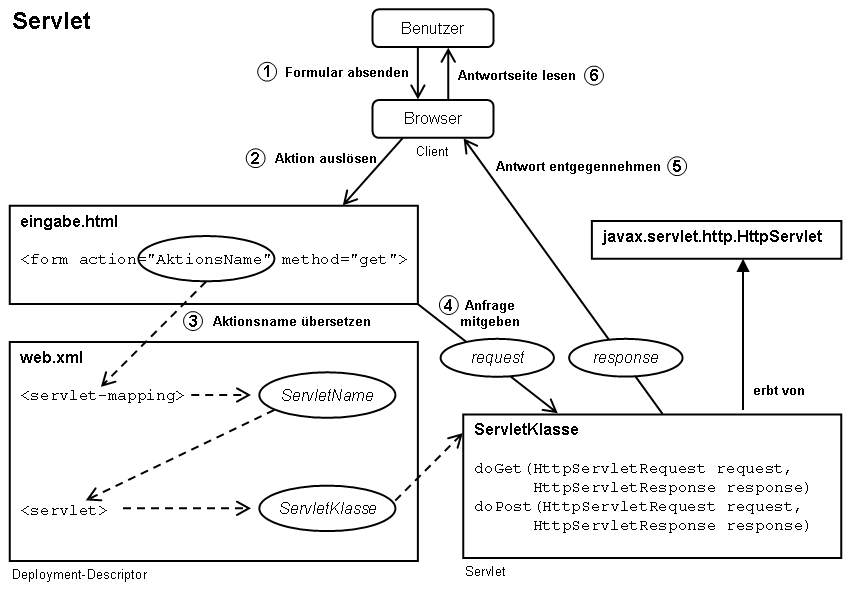
\includegraphics[width=0.9\linewidth]{Bilder/600px-Servlet.png}
	\captionof{figure}[Java-Servlet]{Java-Servlet\footnotemark }
	\label{fig:servlet}
\end{minipage}
\footnotetext{Quelle: \url{https://de.wikipedia.org/wiki/Servlet\#/media/File:Servlet.png}}

Sowohl der Anfangs-, als auch der Endpunkt einer Datenverarbeitung mittels HTML-Formular besteht in dem Client, der mit dem Browser interagiert. Durch diese Interaktion sendet er ein Formular ab, welches daraufhin die gewünschte Aktion auslöst. Dazu muss der Aktionsname jedoch zunächst von einer XML-Datei dahingehend übersetzt werden, dass die entsprechende Initialisierung der ServletKlasse zur Bearbeitung dieser Aktion angesprochen wird.
Sobald dies geschehen ist, erhält die ServletKlasse die Anfrage vom Client, welche sie, entsprechend dem HTML-Formular, mit ihrer doPost- oder doGet-Methode bearbeitet, und schickt die Antwort wiederum dem Browser, welcher diese dem Client anzeigt.

\subsubsection{Einrichtung in Eclipse}
Um eine erfolgreiche Einrichtung eines Java-Servlet mit Eclipse Neo durchführen zu können muss dieses, in der Java EE Version, und Apache Tomcat v 9.0 installiert sein. 
Wenn dies der Fall ist, ist es möglich in Eclipse einen neuen Server einzurichten, \\
\\
\vspace{1em}
\begin{minipage}{\linewidth}
	\centering
	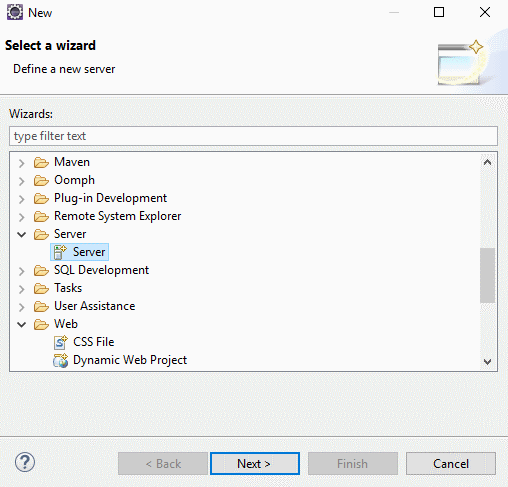
\includegraphics[width=0.7\linewidth]{Bilder/Eclipse-ServerErstellen.png}
    \captionof{figure}[Server einrichten]{Server erstellen}	
	\label{fig:eclipse1}
\end{minipage}
\\
wobei unter dem Ordner Apache die installierte Tomcat Version vorzufinden ist, welche hier  als Servertyp verwendet wird.\\
\\
\vspace{1em}
\begin{minipage}{\linewidth}
	\centering
	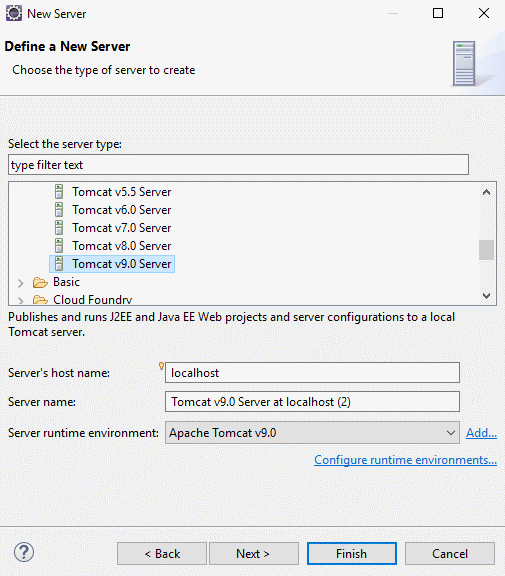
\includegraphics[width=0.7\linewidth]{Bilder/Eclipse-ServerErstellen1.png}
	\captionof{figure}[Server einrichten 2]	{Servertyp festlegen}
	\label{fig:eclipse2}
\end{minipage}
\\

Nachdem dies geschehen ist, muss noch ein Dynamic Web Project eingerichtet und innerhalb desselben, im \glqq Java Resources/src\grqq-  Ordner ein neues Servlet erstellt werden, indem sie nun programmieren können.
\\
\\
\vspace{1em}
\begin{minipage}{\linewidth}
	\centering
	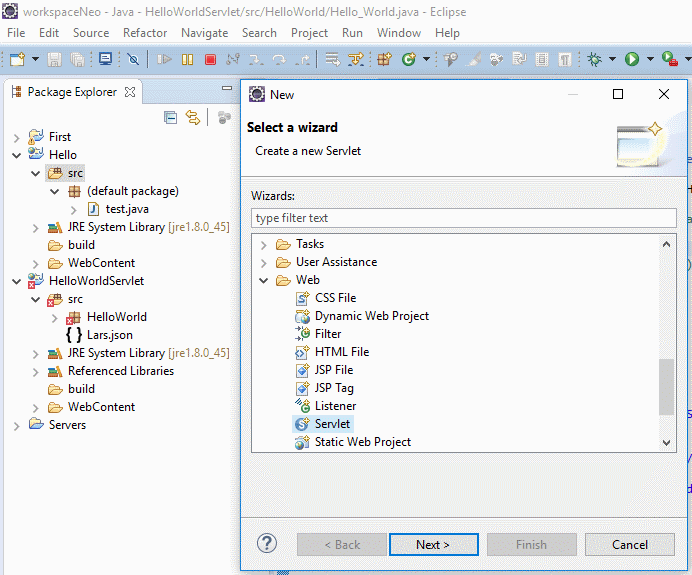
\includegraphics[width=0.7\linewidth]{Bilder/Eclipse-ServerErstellen2.png}
	\captionof{figure}[Servlet erstellen]{Servlet erstellen}	
	\label{fig:eclipse3}
\end{minipage}
\\

Wenn nun aber die Fehlermeldung  \glqq cannot be resolved\grqq{} im Bezug auf die vorgegebenen import-Zeilen auftaucht \\
\\
\vspace{1em}
\begin{minipage}{\linewidth}
	\centering
	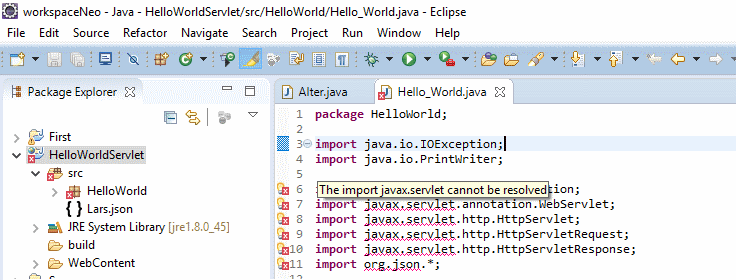
\includegraphics[width=0.9\linewidth]{Bilder/Eclipse-ServerErstellen3.png}
	\captionof{figure}[Fehlermeldung]{Fehlermeldung}	
	\label{fig:eclipse4}
\end{minipage}
\\

muss außerdem noch die servlet-api.jar gedownloadet und über die Eigenschaften des \glqq Dynamic Web Projects\grqq{} unter \glqq Java Build Path\grqq{} in der Kategorie \glqq Libraries\grqq{} mit der Funktion „Add External JARs“ hinzufgefügt werden.\\
\\
\vspace{1em}
\begin{minipage}{\linewidth}
	\centering
	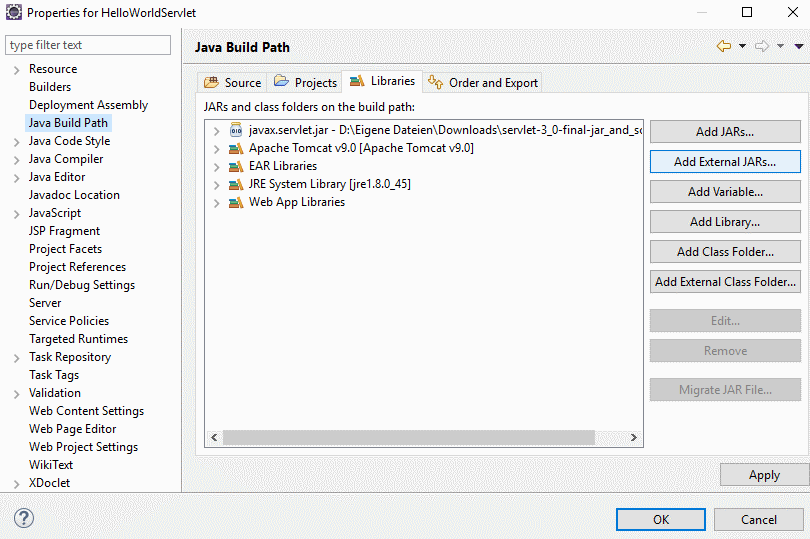
\includegraphics[width=0.9\linewidth]{Bilder/Eclipse-ServerErstellen4.png}
	\captionof{figure}[servlet-api.jar einbinden]{servlet-api.jar einbinden}	
	\label{fig:eclipse5}
\end{minipage}
\\
 

\subsubsection{Implementation}
Die Implementation eines Java-Servlets gestaltet sich, im Vergleich zur Einrichtung eines solchen in Eclipse, eher einfach, da lediglich die doGet-Methode zu befüllen ist, während der restliche Quellcode bereits automatisch erstellt wurde.

So lässt sich beispielsweise mit der Java-Klasse PrintWriter ein HTML-Script in die doGet-Methode schreiben, welches dann beim Aufrufen des Servlets ausgeführt wird:

%\ref{lst:servlet-html}

\vspace{1em}
\begin{lstlisting}[caption=Servlet Beispielcode, label=lst:servlet-html]
protected void doGet(HttpServletRequest request, HttpServletResponse response) throws ServletException, IOException {

	PrintWriter writer = response.getWriter();
	
		writer.println("<html>");
		writer.println("<head>");
		writer.println("<title>");
		writer.println("Hello World");
		writer.println("</title>");
		writer.println("</head>");
		writer.println("<body>");
		writer.println("<h>");
		writer.println("<b>Hello World Servlet</b>");
		writer.println("</h>");
		writer.println("<p>Das ist ein Text</p>");
		writer.println("<a href = Hello_Space> hier </a>");
		writer.println("<br>");
		writer.println("<a href = https://www.google.de target = _blank> Google</a>");
		writer.println("<br>");
		writer.println("Und das auch");
		writer.println();
		writer.println("</body>");
		writer.println("</html>");
		
		writer.close();		
}			
\end{lstlisting}


\vspace{1em}
\begin{minipage}{\linewidth}
	\centering
	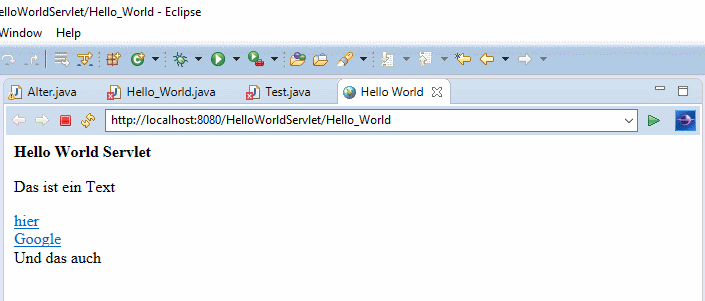
\includegraphics[width=0.9\linewidth]{Bilder/Servlet-Beispiel.png}
	\captionof{figure}[Servlet Beispiel]{Servlet Beispiel}	
	\label{fig:eclipse6}
\end{minipage}
\\

Wie man an diesem Beispiel sehen kann, ist das Servlet nun bereit und muss nur noch mit der gewünschten doGet-Methode befüllt werden.
\subsubsection{Nutzung in unserem Projekt}
In unserem Projekt selber haben wir nicht mit Java-Servlets gearbeitet, sondern haben uns stattdessen für die klassische CGI Schnittstelle, in Form von PHP, entschieden, da Robin bereits ein wenig Erfahrung mit PHP gesammelt hatte, während Java-Servlets absolutes Neuland für uns waren.
Außerdem hat sich PHP für uns alle ein wenig leichter erschlossen, als die Arbeit mit den Servlets, weshalb uns PHP als der sinnvollere Weg erschien.


\subsection{JSON}
\label{sec:JSON}
\emph{Jakob}\\
JSON (= JavaScript Object Notation) ist ein Dateiformat, welches von Programmiersprachen unabhängig ist, weshalb es häufig zum Datenaustausch zwischen verschiedenen Programmiersprachen verwendet wird [Vgl. \cite{json}].

Die Grundlage dieses Formats besteht in 2 Strukturen:

\subsubsection{JSON-Objekt}
\label{sec:JSON-Objekt}
Die erste dieser beiden Strukturen ist das JSON-Objekt, welches dazu dient Zeichenketten Werten zuzuordnen.
Dies kann man sich wie folgt vorstellen:


\vspace{1em}
\begin{minipage}{\linewidth}
	\centering
	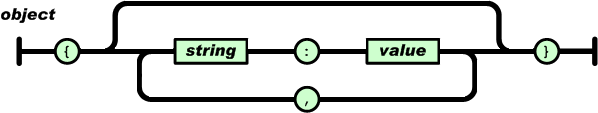
\includegraphics[width=0.9\linewidth]{Bilder/json-object.png}
	\captionof{figure}[JSON-Objekt]{JSON-Objekt\footnotemark }
	\label{fig:json-objekt}
\end{minipage}
\footnotetext{Quelle: \url{http://www.json.org/object.gif}}

Bei der Deklaration eines JSON-Objektes muss lediglich ein Name/Wert-Paar, durch einen \glqq :\grqq{} (Doppelpunkt) getrennt, in die geschweiften Klammern geschrieben werden, um ein Objekt zu deklarieren.
Dabei ist die maximale Anzahl an Name/Wert-Paaren jedoch unbegrenzt. Einem JSON-Objekt können beliebig viele solcher Paare, durch Kommata getrennt, beigegeben werden [Vgl. \cite{json}].

So sähe der Quellcode eines JSON-Objektes beispielsweise wie folgt aus:
\\
\vspace{1em}
\begin{lstlisting}[caption=Lars.json, label=lst:json-objekt]
{
	"Name" : "Lars",
	"Alter" : 17
}
\end{lstlisting}
Hier wird in der Datei \glqq Lars.json\grqq{} ein JSON-Objekt erstellt, welches folgende Name/Wert-Paare beschreibt:
Name = Lars und Alter = 17.

Durch diese einfache Deklaration lässt sich ein JSON-Objekt auch problemlos in anderen Programmiersprachen erstellen, wie hier beispielsweise in JavaScript:
\\
\vspace{1em}
\begin{lstlisting}[caption=JSON-Objekt in JavaScript, label=lst:json-objekt1]
<script>
	var obj = { "Name" : "Lars, "Alter" : 17 };
	var jsonObj = JSON.stringify(obj);
</script>
\end{lstlisting}

oder hier in Java:
\\
\vspace{1em}
\begin{lstlisting}[caption=JSON-Objekt in Java, label=lst:json-objekt2]
import org.json.*;

public void jsonErstellen(){
	JSONObject obj = new JSONObject();
	obj.put("Name", "Lars");
	obj.put("Alter", 17);
}
\end{lstlisting}

Und hier wird die Stärke von JSON deutlich, welche in der Kompatibilität mit sämtlichen Programmiersprachen liegt, wodurch der Datentransfer zwischen diesen deutlich erleichtert wird.

\subsubsection{JSON-Array}
\label{sec:JSON-Array}
Die zweite Struktur, die JSON unterstützt ist das JSON-Array.
Dieses dient, wie für ein Array üblich, der Abspeicherung von Werten, wobei auch eine Verschachtelung mit JSON-Objekten und anderen JSON-Arrays möglich ist [Vgl. \cite{json}].
Dies lässt sich ähnlich, wie das JSON-Objekt, visualisieren:

\vspace{1em}
\begin{minipage}{\linewidth}
	\centering
	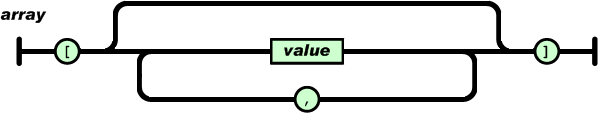
\includegraphics[width=0.9\linewidth]{Bilder/json-array.png}
	\captionof{figure}[JSON-Array]{JSON-Array\footnotemark }
	\label{fig:json-array}
\end{minipage}
\footnotetext{Quelle: \url{http://www.json.org/array.gif}}

Bei der Deklaration eines JSON-Arrays in JSON sind nur zwei Unterschiede zu der eines JSON-Objekts zu beachten, welche zum einen in den äußeren Klammern, die bei einem JSON-Array nicht geschweift sondern eckig sind, und zum andern in dem Inhalt des Arrays bestehen, da in einem Array keine Name/Wert-Paare, sondern nur Werte gespeichert werden.

Die Deklaration eines JSON-Arrays in JSON sähe also beispielsweise so aus:
\\
\vspace{1em}
\begin{lstlisting}[caption=Klasse.json, label=lst:json-array]
[
	{
		"Name" : "Lars",
		"Alter" : 17
	}
,
	{
 		"Name" : "Robin",
 		"Alter" : 17
	}
]
\end{lstlisting}

Und natürlich ist es auch problemlos möglich ein JSON-Array in anderen Programmiersprachen zu deklarieren, jedoch möchte ich an dieser Stelle auf Beispiele verzichten.

\subsubsection{Nutzung in unserem Projekt}
Trotz des einfachen Umgangs mit JSON haben wir uns gegen die Arbeit mit diesem Dateiformat entschieden, was der einfachen Tatsache geschuldet ist, dass wir ein webbasiertes Programm mit einer klassischen CGI-Schnittstelle programmieren wollten, weshalb unsere forcierten Programmiersprachen HTML und PHP waren.
Nun hätten wir zwar den Datentransfer zwischen diesen Sprachen auch mit JSON bewerkstelligen können, jedoch ist dieser zwischen HTML und PHP sowieso durch die Post- und Get-Methoden beider Sprachen [Vgl. [\ref{sec:Formulare}] und [\ref{sec:PHP}]] sehr einfach, weshalb wir an der Stelle diesen Weg eingeschlagen haben.
Jedoch hätten wir JSON benutzt, wenn es unsere Absicht gewesen wäre, die Dateien in der MYSQL-Datenbank abzulegen und nicht nur die Referenz zu der Datei, aber auf dieses Thema wollen wir erst in Kapitel 3 ausführlich eingehen [siehe [\ref{sec:EngineII}]].
\subsection{MYSQL}
\label{sec:MYSQL}
\emph{Jakob}\\
Nachdem obige Thematiken angesichts unseres erneuerten Projektplans irrelevant geworden waren, habe ich mich 
mit MYSQL beschäftigt.
...

\subsubsection{Vorteile}
...

\subsubsection{Datenbank-Entwurf}
Im Folgenden möchte ich auf das Entwerfen einer MYSQL-Datenbank eingehen.
...

\subsubsection{Verwaltung einer Datenbank mit PHP}
Um eine Datenbank in unser Projekt zweckmäßig einzurichten, musste ich mich in eine MYSQL-Einbindung mittels PHP einlesen, welche ich nun darstellen möchte.
...

\pagebreak

% ----------------------------------------------------------------------------------------------------------
% Kapitel 3 - Projekt
% ----------------------------------------------------------------------------------------------------------
\section{Projekt}
\label{sec:Projekt}
\emph{Lars}\\
In diesem Kapitel wird nun unser Projekt dargestellt, indem zunächst das Programm im Gesamten beschrieben wird, woraufhin die einzelnen Teile getrennt dargestellt werden.

\subsection{Datei-Verwaltungs-Programm}
\emph{Lars}\\
Seit Beginn des Projekts im September 2016 sind neun Monate vergangen und das Programm umfasst nun ein Anmeldungsverfahren inklusive Registrationsmöglichkeit, die Möglichkeit Dateien hoch zu laden und nach diesen zu suchen. Im Hintergrund arbeitet ein Server, der sämtliche Anfragen des GUIs annimmt und entsprechend weiter leitet. Zusätzlich verfügt unser Programm über eine Datenbank, welche die Pfade zu den Dateien, sowie ihre Details, also zum Beispiel die Größe und den Dateityp, speichert.

\subsection{GUI}
\label{GUI}
\emph{Lars}\\
GUI ist die Abkürzung für \glqq Graphical User Interface\grqq , was zu Deutsch \glqq Graphische Benutzeroberfläche\grqq{} bedeutet. Als GUI wird also das bezeichnet, was der Benutzer von einem Programm sieht. \\

\subsubsection{Benutzererfahrung}
\label{Benutzererfahrung}
Bei der Verwendung unseres Programms muss sich der Benutzer zunächst anmelden. Das sich öffnende Anmeldefenster kann man in Abbildung \ref{fig:GUIAnmelden} sehen. Falls der Benutzer noch kein Benutzerkonto besitzt kann er sich auch ein solches erstellen. Nach einer Erfolgreichen Anmeldung wird der Benutzer auf die Hauptseite (siehe Abbildung \ref{fig:GUIHauptseite}), den Kern des Programms, weiter geleitet. Hier kann er auf der linke Seite Dateien hochladen, indem er sie entweder per Auswahlfenster öffnet oder per Drag and Drop dem Eingabefeld übergibt. Optional können den hochzuladenden Dateien Beschreibungen hinzufügt werden. Auf der rechten Seite kann der Benutzer seine Dateien, die er bereits hochgeladen hat verwalten. Dazu ist zum Zeitpunkt der Verfassung dieses Texts nur eine Suchfunktion vorhanden. Es werden noch eine Such-, Lösch- und Änderungsfunktion folgen.\\

\vspace{1em}
\begin{minipage}{\linewidth}
	\centering
	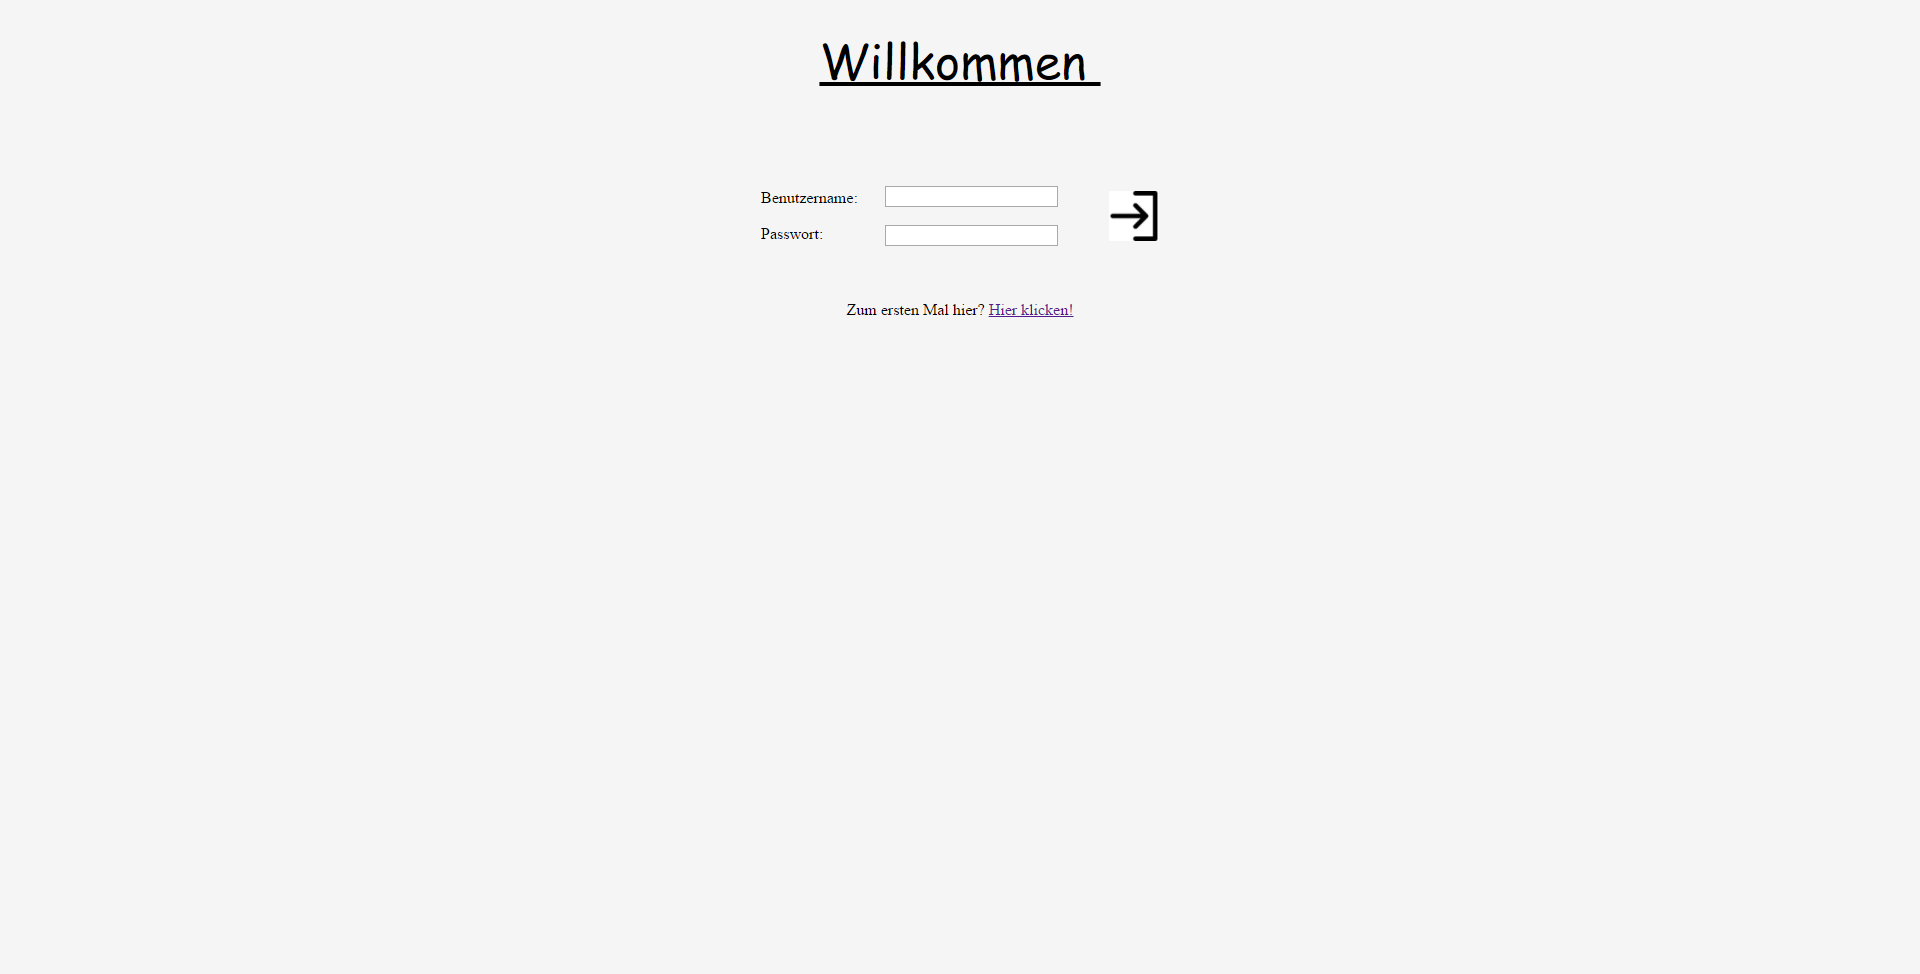
\includegraphics[width=0.7\linewidth]{Bilder/GUIAnmelden.png}
	\captionof{figure}[Aufbau der Anmeldung]{Aufbau der Anmeldung}
	\label{fig:GUIAnmelden}
\end{minipage}

\vspace{1em}
\begin{minipage}{\linewidth}
	\centering
	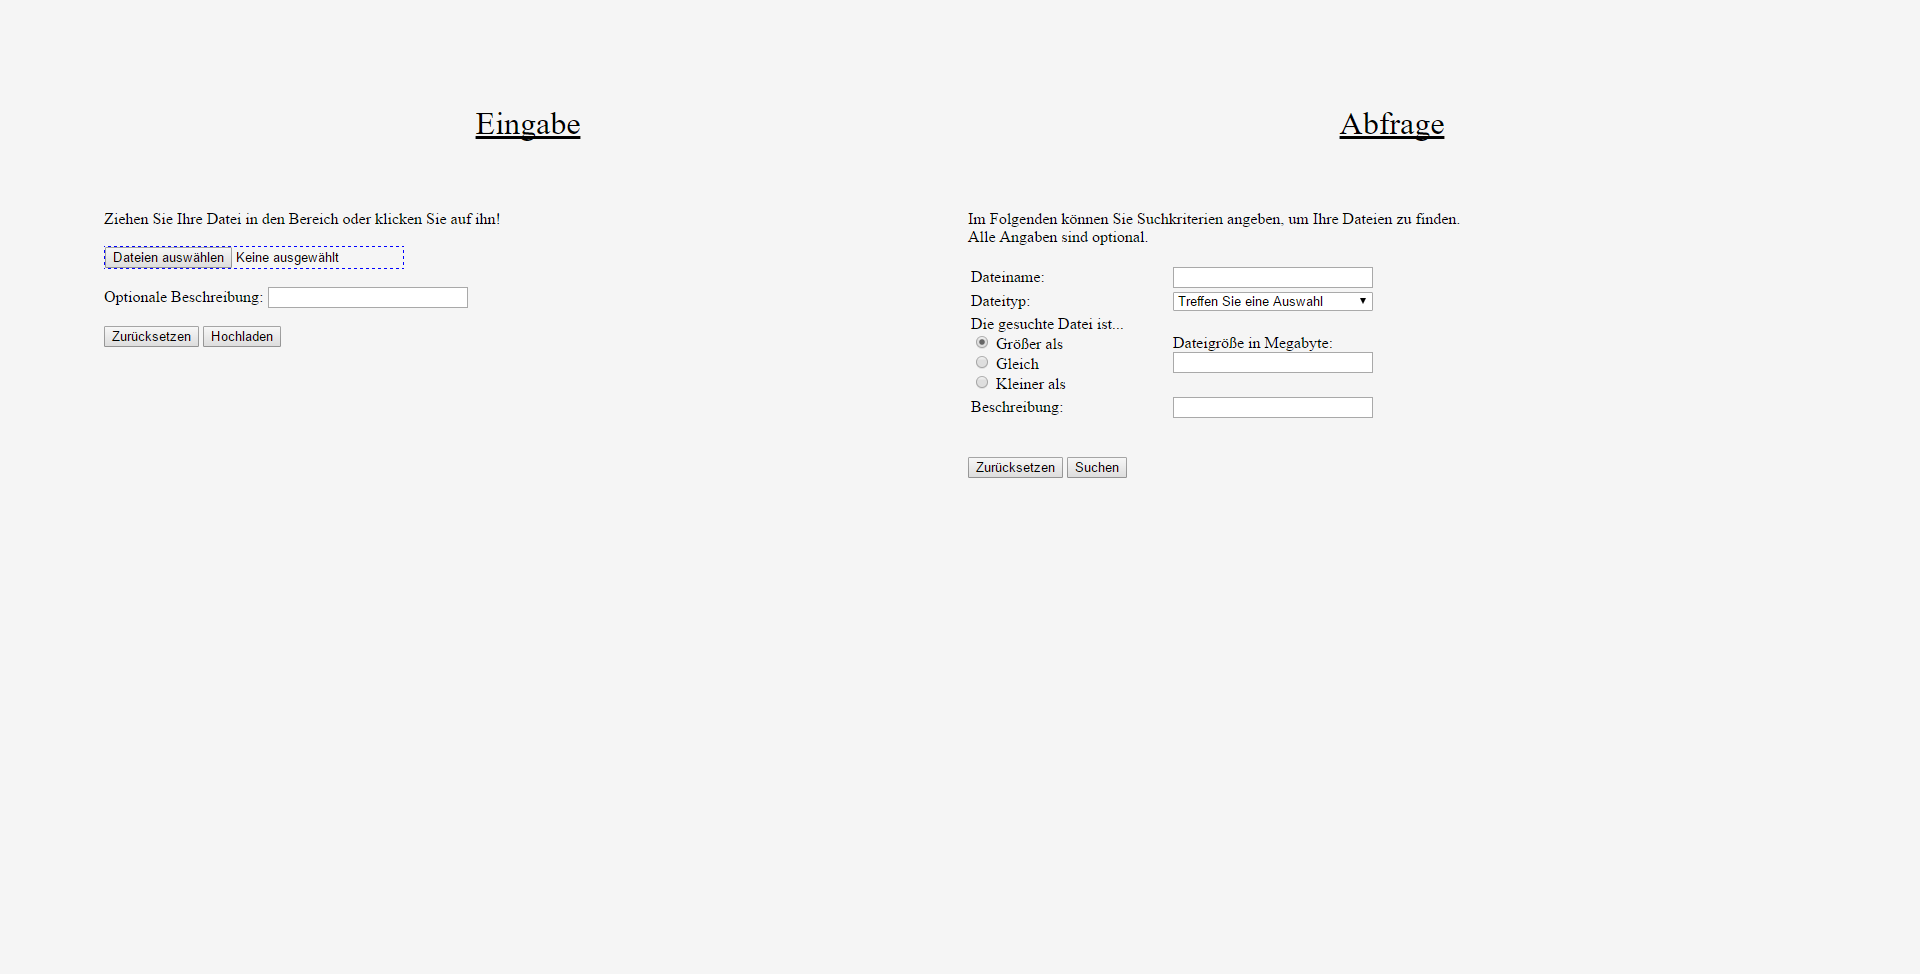
\includegraphics[width=0.7\linewidth]{Bilder/GUIHauptseite.png}
	\captionof{figure}[Aufbau der Hauptseite]{Aufbau der Hauptseite}
	\label{fig:GUIHauptseite}
\end{minipage}
\\

\subsubsection{Realisierung der Hauptseite}
\label{RealisierungHauptseite}
Angefangen hat alles mit einem simplen Quellcode, zum Hochladen einer Datei per HTML. Dieser ist im Folgenden Dargestellt. (Listing \ref{lst:ersterUpload}) Er bestand lediglich aus einer Aufforderung, die Datei, welche der Benutzer hochladen möchte einzufügen, einem Eingabefeld und einem Knopf mit dem Namen \glqq Senden\grqq . Aus diesem Code lernten wir, besonders Ich, wie das Hochladen von Dateien per HTML funktioniert. 

\vspace{1em}
\begin{lstlisting}[caption=Erste Version des Datei-Uploads, label=lst:ersterUpload]
<html>
	<head>
		<title>
			Dateiupload
		</title>
	</head>
	<body>
		Bitte f&uumlgen Sie die Datei ein, die Sie hochladen m&oumlchten!
		<form method="post" action="upload.php" enctype="multipart/form-data">
		Datei:
			<input type="hidden" name="MAX_FILE_SIZE" value="100000">
			<input type="file" name="datei" size="40" maxlength="100000">
			<input type="submit" name="Submit" value="Senden">
		</form>
	</body>
</html>
\end{lstlisting}

Nach Sammlung von Inspiration auf der Internetseite \url{https://jqueryui.com} wurde die Hauptseite [\ref{fig:GUIHauptseite}] entworfen und programmiert. Zunächst war die Idee, unterhalb der Eingabe und Abfrage das Suchergebnis ausgeben zu lassen. Dies stellte sich aber als eher unpraktisch heraus, weshalb wir beschlossen, das Frame [\ref{sec:Frames}], was zuvor nur die Abfrage enthielt, nun auch das Suchergebnis ausgeben zu lassen. Der Plan war nun also grob gesagt, mithilfe des Formulars [\ref{sec:Formulare}], das die Suchabfrage aufnimmt, auf ein PHP-Dokument [\ref{sec:PHP}] zu verweisen, welches schlussendlich das HTML-Dokument[\ref{sec:HTML}] mit dem Ergebnis aufruft. \\

\subsubsection{Realisierung der Anmeldung}
\label{RealisierungAnmeldung}
Mit der Zeit entstand die Idee der Gestaltung eines Anmeldeverfahrens. Dieses sollte aus einem Benutzernamen und einem Passwort bestehen. Als die Anmeldung funktionierte fiel uns auf, dass natürlich auch eine Registrierung notwendig sein wird. Auch sie besteht aus einem Feld, zur Eingabe eines Benutzernamens. Jedoch beinhaltet die Registrierung zwei Felder für die Eingabe des Passworts, um zu gewährleisten, dass sich der Benutzer dass richtige Passwort auch tatsächlich merkt oder zumindest notiert. Der Nachteil beim einmaligen Eintippen des Passworts bei der Registrierung ist, dass der Benutzer sich eventuell vertippen kann, sich also ein falsches Passwort merkt beziehungsweise notiert und somit später keinen Zugriff mehr auf seine Dateien erhält.

\subsection{Engine I: Interface und Datei-System}
\emph{Robin}\\
Dieser Teil der Engine ist für den Upload zuständig. Die "upload.php"-Datei bekommt die hochzuladene Datei durch eine POST-Methode von der "eingabe.html"-Datei. Die Uplaod datei ließt nun die benötigten Daten aus der Datei heraus wie z.B. Name, Größe, Datei-Typ und Erstellung-/Änderungsdatum. Diese Informationen werden dann zusammen mit dem neuen Pfand in der Datenbank abgespeichert. Danach wird die "eingabe.html"-Datei wieder aufgerufen um wieder auf den vorherigen Frame zu kommen.
Zunächt war geplant, die "upload.php"-Datei in die "eingabe.html" zu integrieren, doch später habe ich mich dazu entschieden, den Upload extern zu machen, da es so einfacher zu schreiben ist und übersichtlicher in der Datei selbst.


\subsection{Engine II: Interface und Datenbank}
\emph{Jakob}\\
Darstellung Interface und Datenbank...
\pagebreak
% ----------------------------------------------------------------------------------------------------------
% Kapitel
% ----------------------------------------------------------------------------------------------------------
\section{Fazit}
\label{sec:Fazit}
\emph{Lars}\\
Im Folgenden wird jeder von uns ein Fazit geben, indem er darstellt, was er aus dem Projekt gelernt hat, Dinge die ihm gefielen und so weiter.

\subsection{Lars}
Im Verlaufe des Projektes habe ich festgestellt, dass mir das Programmieren sehr viel Spaß macht und ich mich auch nach der Schule in Richtung IT orientieren werde. Ferner stellte ich fest, dass Teamarbeit nicht sehr leicht ist, insbesondere, wenn jedes Gruppenmitglied prinzipiell den Anderen gegenüber gleich gestellt ist, es also kurz gesagt keine festgelegte Gruppenleitung gibt. Mit der Zeit kristallisieren sich zwar Personen heraus, die die Leitung übernahmen, jedoch entstand dann das Problem, dass diese nicht über ausreichend Autorität verfügten, als dass sie die anderen Gruppenmitglieder hätten sanktionieren können, wenn diese ihre Aufgaben nicht erfüllten. Insgesamt empfand ich die Arbeitsatmosphäre als sehr angenehm, da uns sehr viele Freiheiten gelassen wurden und es keine festen Vorgaben gegeben hat, an die wir halten mussten.

\subsection{Robin}
...

\subsection{Jakob}
Wie bereits eingangs mehrfach erwähnt, bestand die Schwierigkeit von unserem Projekt, meiner Meinung nach, nicht in der Thematik, sondern in der Arbeit miteinander. Dadurch, dass wir zu dritt an einem solchen Projekt, welches viel größer ist, als alles Andere, was wir bis dahin programmiert haben, gearbeitet haben, sind wir auf 2 Ebenen auf ganz neuem Terrain gewandert.
Zum einen war natürlich die Thematik und die Art des Programmierens für uns absolut ungewohnt.
Viel schwerwiegender war jedoch die Tatsache, dass wir bis dato noch nie so frei an einem Projekt gearbeitet haben, welches es gemeinsam zu verfolgen galt.
Und genau in den Problemen, die daraus entstanden, sehe ich den größten und essentiellsten Lerneffekt, den wir mitnehmen sollten.
Denn in diesem Schuljahr konnten wir einen ersten Blick in das Leben nach der Schule werfen, durften feststellen, wie es ist nicht mehr an der Hand gehalten und behütet durch die Aufgaben geführt zu werden.
Wir mussten uns zwar erst langsam an diese Situation gewöhnen und haben letztendlich auch kein großartiges Projekt auf die Beine stellen können, jedoch bin ich froh und dankbar, dass ich diese Erfahrung des \glqq Unbehütet-Seins\grqq{} in einer behüteten Umgebung machen durfte.
Aus diesem Grund bin ich froh mich für diesen Projektkurs entschieden zu haben und überzeugt davon, dass er uns besser auf das \glqq richtige Leben\grqq{} vorbereitet hat, als so manch anderes Fach, wenn man bereit ist sich seine Fehler einzugestehen und daraus Konsequenzen zu ziehen.

\pagebreak
% ----------------------------------------------------------------------------------------------------------
% Literatur
% ----------------------------------------------------------------------------------------------------------


\renewcommand\refname{Literaturverzeichnis}
\bibliographystyle{alpha}
\bibliography{bibo}
\pagebreak


% ----------------------------------------------------------------------------------------------------------
% Anhang
% ----------------------------------------------------------------------------------------------------------
\pagenumbering{Roman}
\setcounter{page}{1}

\lhead{Anhang \thesection}
\begin{appendix}

\section*{Anhang}
\phantomsection
\addcontentsline{toc}{section}{Anhang}
\addtocontents{toc}{\vspace{-0.5em}}


\end{appendix}


\newpage
\thispagestyle{empty}
\begin{center}
	\vspace*{5em}
	\huge\textbf{Erklärung}\\
\end{center}
\vspace{2em}
Hiermit versichere ich, Jakob Fleischer, dass ich meinen Anteil an unserer Dokumentation selbständig verfasst und keine anderen, als die angegebenen Quellen und Hilfsmittel benutzt habe.

\vspace{4em}
\begin{minipage}{\linewidth}
	\begin{tabular}{p{15em}p{15em}}
		Datum: &  .......................................................\\
		& \centering (Unterschrift)\\
	\end{tabular}
\end{minipage}



\newpage
\thispagestyle{empty}
\begin{center}
	\vspace*{5em}
	\huge\textbf{Erklärung}\\
\end{center}
\vspace{2em}
Hiermit versichere ich, Robin Schlaak, dass ich meinen Anteil an unserer Dokumentation selbständig verfasst und keine anderen, als die angegebenen Quellen und Hilfsmittel benutzt habe.

\vspace{4em}
\begin{minipage}{\linewidth}
	\begin{tabular}{p{15em}p{15em}}
		Datum: &  .......................................................\\
		& \centering (Unterschrift)\\
	\end{tabular}
\end{minipage}

\newpage
\thispagestyle{empty}
\begin{center}
	\vspace*{5em}
	\huge\textbf{Erklärung}\\
\end{center}
\vspace{2em}
Hiermit versichere ich, Lars Schmalbach, dass ich meinen Anteil an unserer Dokumentation selbständig verfasst und keine anderen, als die angegebenen Quellen und Hilfsmittel benutzt habe.

\vspace{4em}
\begin{minipage}{\linewidth}
	\begin{tabular}{p{15em}p{15em}}
		Datum: &  .......................................................\\
		& \centering (Unterschrift)\\
	\end{tabular}
\end{minipage}
\end{document}


%Die Quellen befinden sich in der Datei \textit{bibo.bib}. Ein Buch- und eine Online-Quelle sind beispielhaft eingefügt. [Vgl. \cite{buch}, \cite{online}]
%Abkürzungen lassen sich natürlich auch nutzen (\ac{OSGi}). Weiter oben im Latex-Code findet sich das %Verzeichnis.


%Beispiele
%
%
%----------Listings----------
%
%
% \ref{lst:arduino}.
%
%\vspace{1em}
%\begin{lstlisting}[caption=Arduino Beispielprogramm, label=lst:arduino]
%int ledPin = 13;
%void setup() {
%    pinMode(ledPin, OUTPUT);
%}
%void loop() {
%    digitalWrite(ledPin, HIGH);
%    delay(500);
%    digitalWrite(ledPin, LOW);
%    delay(500);
%}
%\end{lstlisting}
%
%
%
%----------Aufzählung----------
%
%
%\begin{compactitem}
%	\item Nur
%	\item ein
%	\item Beispiel.
%\end{compactitem}
%
%
%
%----------Tabelle----------
%
%
%\vspace{1em}
%\begin{table}[!h]
%	\centering
%	\begin{tabular}{|l|l|l|}
%		\hline
%		\textbf{Name} & \textbf{Name} & \textbf{Name}\\
%		\hline
%		1 & 2 & 3\\
%		\hline
%		4 & 5 & 6\\
%		\hline
%		7 & 8 & 9\\
%		\hline
%	\end{tabular}
%	\caption{Beispieltabelle}
%	\label{tab:beispiel}
%\end{table}
%
%
%
%----------Grafik/Abbildung----------
%
%
%\vspace{1em}
%\begin{minipage}{\linewidth}
%	\centering
%	\includegraphics[width=0.7\linewidth]{Bilder/layering-osgi.png}
%	\captionof{figure}[OSGi Architektur]{OSGi Architektur\footnotemark }
%	\label{fig:osgi}
%\end{minipage}
%\footnotetext{Quelle: \url{http://www.osgi.org/Technology/WhatIsOSGi}}



%section*{}  -> Section, die nicht im Inhaltsverzeichnis aufgeführt wird



